\section{Response of the epipelagic community to extreme El Niño events}

This section describes the simulated response of the epipelagic community to ENSO as a function of organisms' size and analyses the underlying mechanisms. Here, we focus on  the marine ecosystem response to the three strongest El Niño events in the historical record, namely those of 1982/83, 1997/98 and 2015/16 \citep{santosoDefiningCharacteristicsENSO2017}. During these events, the central and eastern Pacific has warmed by more than 2°C (Fig\ref{fig:nemo-had-sst}a), displacing the warm waters and associated atmospheric convection from the western to the central Pacific. The atmospheric signature of these El Niño had dramatic climatic consequences, including droughts and wildfires, in countries bordering the western Pacific, but also torrential rains and flooding along the south American coast \citep{caiClimateImpactsNino2020}. Their oceanic signature also tremendously impacted marine ecosystems and biodiversity, leading to major disruption of marine life and seabird populations \citep{valleImpact198219831987}, promoting large-scale marine heatwaves \citep{holbrookKeepingPaceMarine2020} and coral bleaching \citep{claarGlobalPatternsImpacts2018}.  The response of the ocean during each of these three extreme events has been extensively described and analyzed in terms of physics  (e.g. \citealp{philanderChapter33Simulation1985, lengaigneOceanResponseMarch2002, puyModulationEquatorialPacific2019}), biogeochemistry (e.g. \citealp{barberBiologicalConsequencesNino1983, chavezBiologicalChemicalResponse1999, strammaObservedNinoConditions2016}) and marine ecosystems \citep{glynnNINOSOUTHERNOSCILLATION198219831988, glynnCoralBleachingMortality2001, eakin20142017Globalscale2019} 

In order to isolate the generic response of epipelagic communities to extreme El Nino events, independent of the intrinsic characteristics of each event, we perform a composite analysis of these three extreme events, averaging monthly anomalies of temperature, ocean velocity, low-trophic level concentrations (LTL, i.e. phyto and zooplankton, particulate organanic matter) and epipelagic commnunity biomass over the periods 1982-1984, 1997-1999 and 2015-2017. These extreme El Niño events are also followed by La Niña conditions in the following year (more intense in the case of the 1997/98 event), which also allows for a discussion epipelagic community response mechanisms to La Niña events. Although the temporal evolution and amplitude of the processes discussed below vary slightly between events, the relative importance of the processes discussed in our composite analysis remains the same when these three extreme events are analyzed individually (not shown). 

\subsection{Modeled upper-ocean response: from physics to ecosystems}

Because these are major environmental drivers of the epipelagic community biomass variability, we first describe in Figure \ref{fig:hov_nemo_ape}a-c the temporal evolution of monthly equatorial anomalies of the upper ocean temperature, chlorophyll concentrations and zonal currents during and after extreme El Niño events, in the form of equatorial time-longitude diagrams, whose time of origin is the January month before the onset of the El Nino event. The warming signal associated with El Niño begins in the central equatorial Pacific in early spring, spreads rapidly to the eastern Pacific, intensify during the summer and fall, peaks at the end of the calendar year, and finally rapidly declines and transitions to La Niña conditions the following spring (month 16, Fig.\ref{fig:hov_nemo_ape}a). The development phase of El Niño is also characterized by strong  eastward surface currents anomalies in the western and central Pacific (Figure \ref{fig:hov_nemo_ape}c) induced by anomalous westerly winds, promoting warming of the the central Pacific and eastward movement of the warm-pool to the eastern equatorial Pacific. These current anomalies reverse at the peak of El Niño and during La Niña. The simulated plankton concentration anomalies largely mirror those of temperature, with a strong decline during El Niño and an increased bloom during La Niña (Figure \ref{fig:hov_nemo_ape}.b). 


\begin{figure}[h!tp]
	\centering
	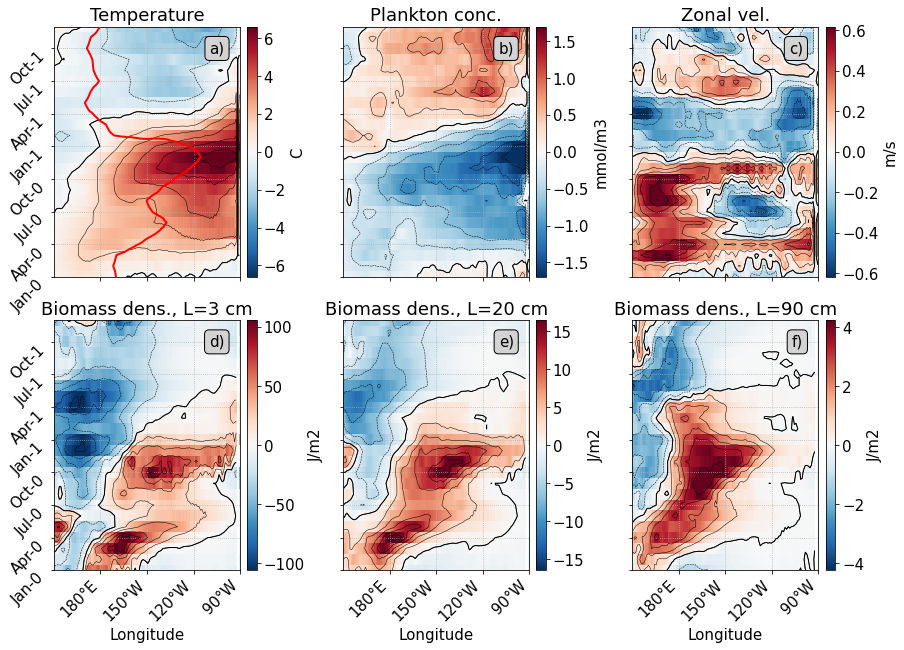
\includegraphics[scale=0.4]{plot_all_hovmoller_phys_oope.png}	
	\caption{Hovmoller diagrams of equatorial temperature (a), low-trophic level concentrations (b), zonal velocity (c) and fish biomass anomalies (3cm, 20cm and 90 cm in d, e, f, respectively).}	
	\label{fig:hov_nemo_ape}
\end{figure}

A similar analysis is then performed for epipelagic biomass for the three size classes we selected (Fig\ref{fig:hov_nemo_ape}d, Fig\ref{fig:hov_nemo_ape}e and Fig\ref{fig:hov_nemo_ape}f). Their responses to El Niño share some common features: positive biomass anomalies appear near the dateline at the beginning of the the calendar year and propagate eastward toward the central Pacific until late spring (May/June). This positive biomass anomalies in the central Pacific re-intensify in fall and quickly disappear in winter. They are also accompanied by a decrease in biomass in the western Pacific from the summer of the El Niño year. These negative anomalies persist after the El Niño peak and during the subsequent La Niña event but remain largely confined to the western Pacific. However, there are significant differences in the behaviour of the three size classes, including a westward-shifting response size classes increase.

The analysis of the trend terms (equation \ref{eq:apecosm_trend}) allows us to identify the role of the processes responsible for the response of the epipelagic community to El Niño highlighted in Figure \ref{fig:hov_nemo_ape} by analysing the associated tendency terms (equation ??). The same hovmuller diagrams are made for the main trend terms (right members of \ref{eq:apecosm_trend}) and for their integral representing their contribution to the total biomass change. We also analyze various key parameters of the biological response to changing environmental conditions, namely growth rate ($\gamma$ in equation \ref{eq:apecosm_trend}), functional response and predation mortality rates ($M$ in equation \ref{eq:apecosm_trend}). Because the relative importance of these processes varies with the size classes, these analyses are discussed separately for each size class.

\subsection{Processes driving epipelagic upper-ocean response}

Figure \ref{fig:fig7} presents a synthesis of the respective contribution of biological (i.e. the combined action of growth and predation) and physical (i.e. the combined action of advection and diffusion) processes on the epipelagic biomass response to ENSO for three size classes. For the largest size class, physical processes (Fig \ref{fig:fig7}i) explain most of the biomass changes (Fig \ref{fig:fig7}g), with biological processes being an order of magnitude smaller (Fig \ref{fig:fig7}h). The increase in biomass in the central Pacific and decrease in the west is consistent with passive transport of large organisms by ocean currents from the western to the central Pacific. This advection is due to the strong eastward current anomalies simulated in the western and central Pacific during the onset and development phase of an extreme El Niño (up to 0.6m/s; see Fig\ref{fig:hov_nemo_ape}c). While the influence of passive horizontal transport by currents dominates active movements and is broadly similar for all size classes, the relative importance of biological processes increases as fish size decreases. The decrease in biomass in the western Pacific is indeed primarily the result of biological processes for intermediate and small size classes. In the central and eastern Pacific, the combined action of dynamical and biological processes explain biomass increase during El Niño (Fig \ref{fig:fig7}a-f) while these processes largely cancel each other when the equatorial Pacific reverses to La Niña conditions, resulting in small biomass changes in this region. There are two main reasons why the relative importance of biological processes decreases with increasing size. First, predation is size-based in APECOSM, resulting in high predation pressure on small organisms, which decreases with size since larger organisms have no predators in the model. The second important biological process that affects biomass is growth, which includes a flux term and a source term (see equation \ref{eq:apecosm_trend}) that are both temperature-dependent. The source term controls biomass production. It varies as ${\gamma}/{w}$, which scales linearly with $w^{-\frac{1}{3}}$ and thus decreases sharply with size.


\begin{figure}[h!tp]
	\centering
	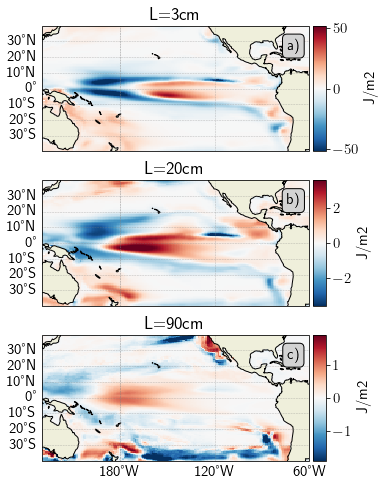
\includegraphics[scale=0.4]{figs/fig7.png}	
	\caption{Total (left), biologically (predation and growth, middle) and dynamically (right, advection and diffusion) induced changes in fish biomass for small (top), intermediate (middle) and large (bottom) sizes.}
	\label{fig:fig7}
\end{figure}

The influence of dynamical processes is simple. It results from the transport of biomass from the western to the central Pacific due to the strong eastward currents appearing during extreme El Niño conditions. It is experienced by all size organisms. The significant and sometimes dominant contribution of biological processes for small and medium size classes is, however, more difficult to understand intuitively as it results from the combined action of predation mortality and growth. Therefore, we further detail the respective contribution of predation and growth and their driving factors for small and medium size classes on Figures \ref{fig:fig8} and \ref{fig:fig9} respectively. For small size classes (3cm), the effects of predation mortality balance the effects of growth (Fig. \ref{fig:fig8}a and Fig. \ref{fig:fig8}.b), which results in a net effect of biological processes two to three times smaller than the effect of physical processes (Fig. \ref{fig:hov_nemo_ape}d). Growth leads to an increase  of biomass in the central Pacific (between dateline and 150\degree{}W) at the onset of El Niño, expanding eastward until its peak. These positive biomass anomalies then decrease slightly during the following La Niña conditions. This evolution can be related to the evolution of the modeled growth rate, which increases in the central and eastern Pacific during El Niño and decreases slightly during the following La Niña, matching closely the evolution of temperature. Since changes in growth rate are largely driven by temperature, the anomalous warming observed east of the dateline during El Niño increases the growth rate and thus the biomass of small size classes due to the source term associated to growth in equation (1). Conversely, the cooling observed during the subsequent La Niña conditions decreases the growth rate, dampening the El Niño-induced increase in biomass. In contrast to the central and eastern Pacific, the growth rate decreases in the cooling western Pacific from June of the El Niño year and this contributes to a decrease in biomass, which reverts during the following La Niña. Again, temperature changes have a major influence on growth rate and biomass of small size class organisms. Despite its importance in controlling growth and reproduction, Fig. \ref{fig:fig8}.e shows that the functional response is indeed not the main driver here, as its influence is two orders of magnitude smaller than the the temperature-driven biomass changes induced by growth. The functional response show negative anomalies that are consistent with the reduction of low-trophic level prey concentrations modulated by temperature, which controls the swimming speed of predators (attack rate of the Holling type 2 functional response), and the vertical distribution and swarming level of low trophic level prey, which control their availability to predators. As mentioned earlier, changes in biomass induced by predation largely mirror those induced by growth. They act to decrease biomass in the central and eastern Pacific and increase it in the western Pacific, closely following the biomass changes of intermediate size predators. Despite their opposite effect on biomass, the effects of growth dominate those of predation, explaining most of the decrease of small sized biomass in the western Pacific during El Niño and the subsequent La Niña and enhancing the biomass increase in the central Pacific induced by dynamical processes during El Niño.  

\begin{figure}[h!tp]
	\centering
	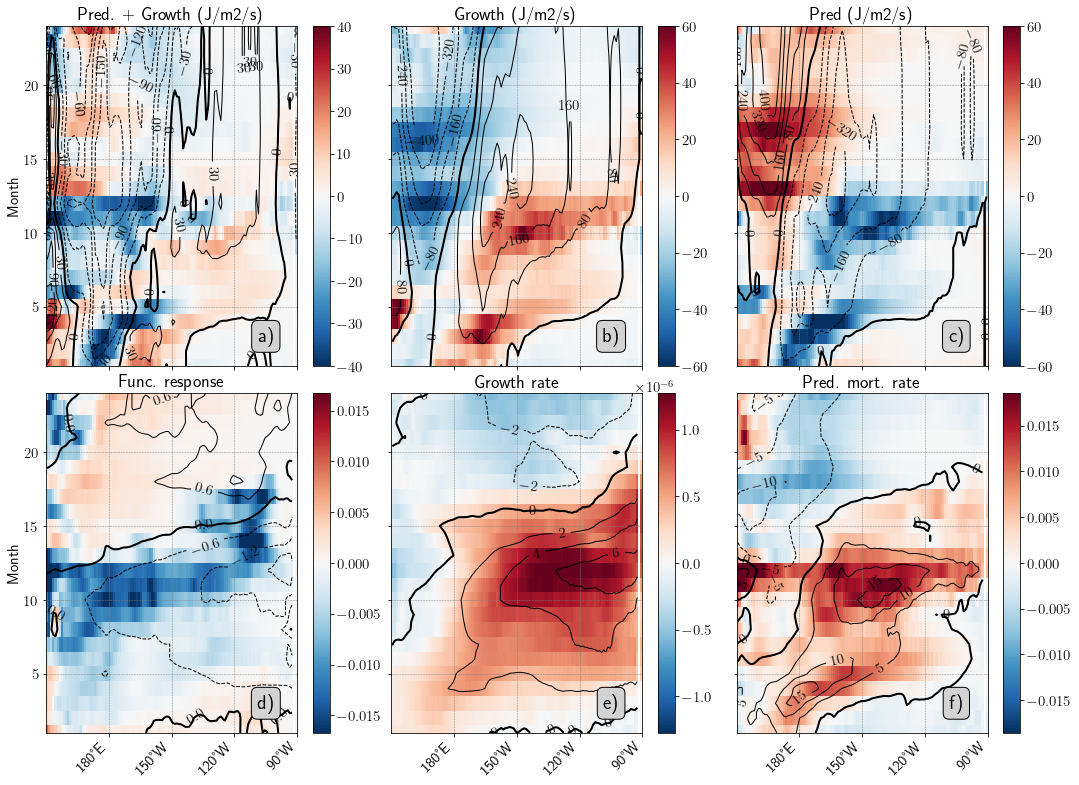
\includegraphics[scale=0.4]{figs/fig8.png}	
	\caption{Small sizes biological trends (colors) and time-integrated trends (contours) (a, b and c). Functional response (colors) and plankton (contours) anomalies (d). Growth rate (colors) and temperature (contours) anomalies (c). Predation mortality rate (colors) and intermediate biomass anomalies (f).}
	\label{fig:fig8}
\end{figure}

Biomass changes induced by growth and predation for intermediate size classes are similar to those simulated for small size classes: they are opposite and of the same order of magnitude but overall, the effects of growth dominate those from predation. Growth increases fish biomass in the central Pacific from the onset to the peak of El Niño, while it decreases the biomass in the western Pacific during the subsequent La Niña. However for intermediate size classes, the influence of temperature on fish physiology is not anymore the dominant factor of biomass changes from biological processes as it was for small organisms. As opposed to small size classes, growth rate changes reflect changes in the functional response, which increases in the central Pacific both because of warmer waters (increasing swimming speed that controls the attack rate parameter in the functional response) and increased food availability due to the increase of small organisms' biomass. These processes contribute to increasing the biomass of intermediate size organisms. In the western Pacific, the growth rate doesn't change much (Fig. \ref{fig:fig7}b). This is because the intermediate size organisms change their vertical distribution (from around 60m to around 30m, cf. Fig. \ref{fig:fig8}e) pushed by the shallowing of the thermocline and concentrate at the depth of their prey so that they do not experience neither substantial prey changes (Fig.\ref{fig:fig8}d) nor water cooling (Fig.\ref{fig:fig8}a). The source component of growth is therefore not changed but the advective flux along the weight axis (see equation \ref{eq:apecosm_trend}) decreases during La Niña (Fig. \ref{fig:fig7}a) because of the biomass decrease induced both by passive eastward advection by marine currents during El Niño and increased mortality rates (Fig. \ref{fig:fig7}d). However, predation acts to dampen the effects of growth, reducing biomass in the central Pacific because of increased predation by large size classes there and increasing biomass in the western Pacific during the subsequent La Niña because of reduced predation. The changes induced by the combination of both processes is dominated by growth however and resembles the one obtained for small sizes albeit a modest westward shift. As for small sizes, the biomass decrease in the western Pacific during El Niño and the subsequent La Niña is largely driven by a growth reduction, while dynamical processes dominate the biomass increase east of the dateline with a smaller contribution from growth.  The comparison of active and passive velocities suggests that passive movements (i.e. advection by the ocean currents) dominate, with ocean current anomalies greater than active velocity anomalies by a factor of $\approx\ 20$.

\begin{figure}[h!tp]
	\centering
	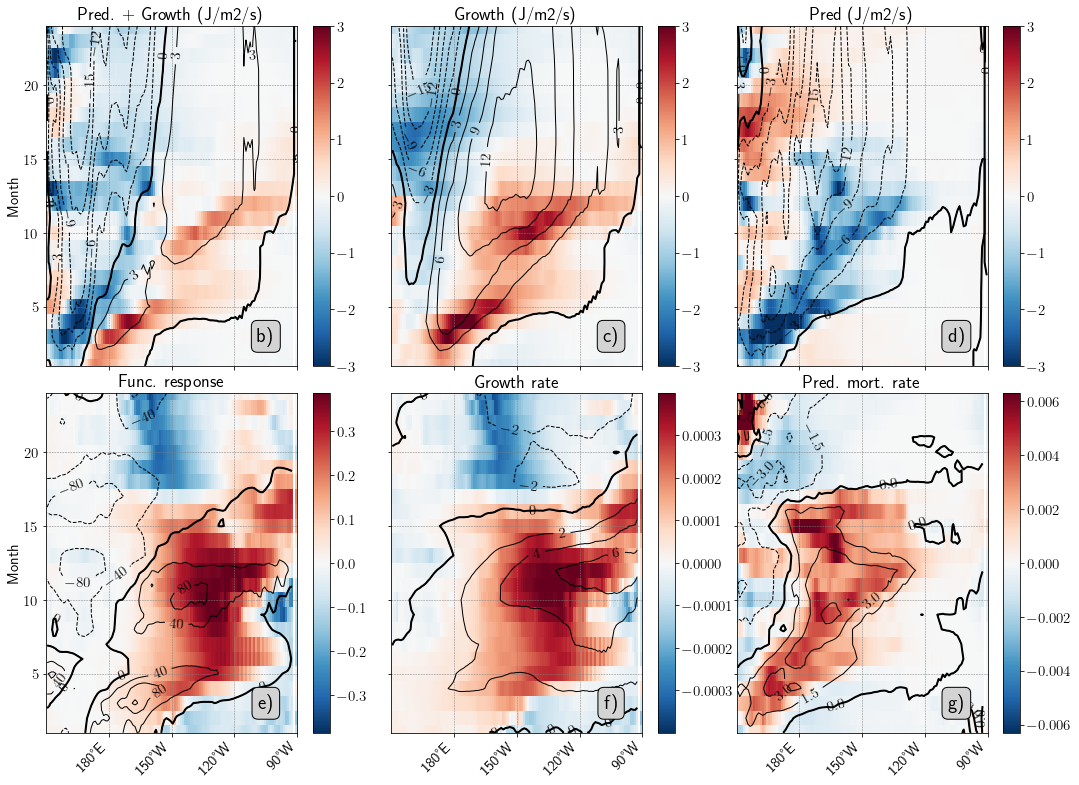
\includegraphics[scale=0.4]{figs/fig9.png}	
	\caption{Intermediate sizes trends (colors) and time-integrated trends (contours) for growth and predation (a and b). Growth rate (colors) and temperature (contours) anomalies (c). Predation mortality rate (colors) and large biomass anomalies (d). Functional response (colors) and small biomass (contours) anomalies (f).}	
	\label{fig:fig9}
\end{figure}

Changes in large fish biomass are dominated by advection/diffusion transport processes, while predation and growth have virtually no impact because their importance decreases structurally with size (see above). 

%ADD HERE A SMALL PARAGRAPH SUMMARIZING THE DOMINANT PROCESSES DRIVING BIOMASS SHIFT FOR ALL SIZE CLASSES.

\subsection{Subsurface response}

Figure \ref{fig:profiles} shows the mean equatorial profiles for temperature, zonal velocity, low-trophic level concentration and fish-biomass (contour lines) and the composites of OND El Nino anomalies. Mean temperature exhibits a deep thermocline in the western Pacific and a shallow one in the east, which flattens during El Nino, leading to a warming in the east and a cooling in the west. The structure of the Equatorial Undercurrent is clearly visible on the zonal velocity profile. It strongly weakens during El Nino, while strong positive (i.e. eastward) anomalies occur near the surface. Low-trophic level biomass is maximum in the top 50m of the eastern Pacific and decrease during El Nino, due to the flattening of the thermocline, which is associated with a decrease in nutrient supply.

Right columns of Fig \ref{fig:profiles} show the equatorial profiles of fish biomass density for the three size-classes under focus here. On average, biomass in the western Pacific reaches $100m$, while in the eastern Pacific, it remains very close to the surface $25m$. The western biomass for small sizes is maximal close to the surface near the dateline, while for intermediate and large sizes, the maximum occurs deeper, around $40m$ in the western Pacific (between 150 and 160\degree{}E)
During El Nino conditions, fish biomasses increase in the eastern Pacific (except very close to the surface) and a decrease in the west. However, the latter is not homogeneous on the vertical, since strong positive anomalies appear around 40m in the east for intermediate and large sizes. These are induced by a tightening of the vertical habitat, due to the shallowing of the thermocline.

\begin{figure}[h!tp]
	\centering
	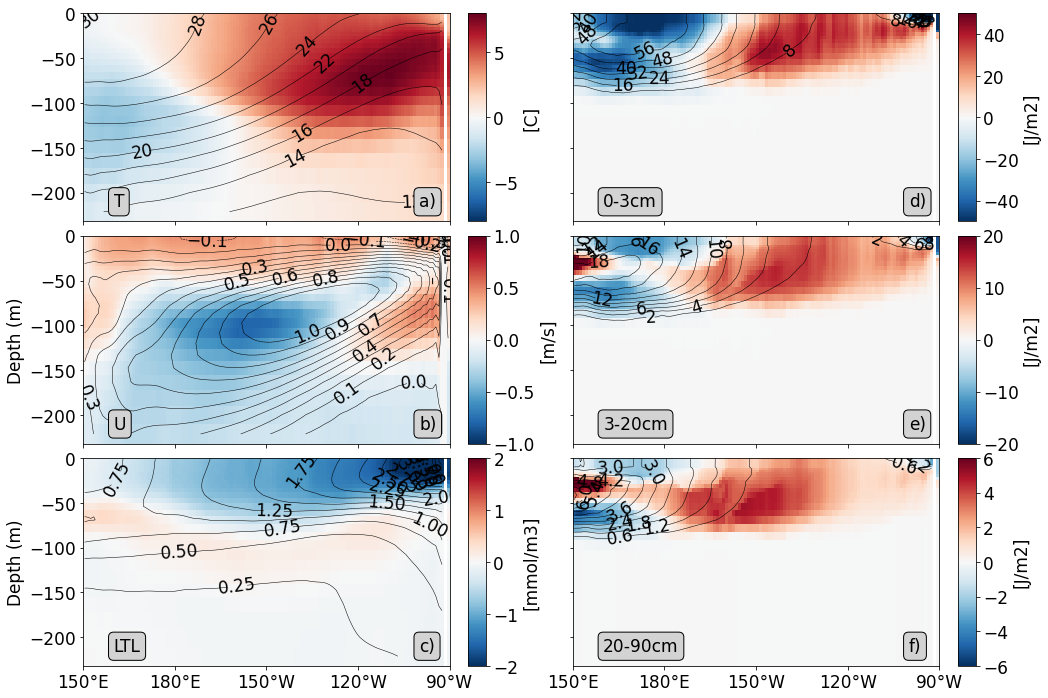
\includegraphics[scale=0.4]{figs/forage_mean_ond97.png}	
	\caption{Pacific equatorial profiles of temperature (a), zonal velocity (b), low-trophic concentration (c) and fish biomass (d for small, e for intermediate and f for large sizes). Mean are represented as black contour lines and El Nino anomalies are represented in colors.}	
	\label{fig:profiles}
\end{figure}

\subsection{Generalization}

Figure \ref{fig:mean_ond97_ape} shows that, in average, small epipelagic fish biomass is maximal around 5\degree{}N and 5\degree{}S (see the $2.0$ contour Fig \ref{fig:mean_ond97_ape}a), while smaller biomasses are found at the equator and in the eastern Pacific. During El Nino, anomalies calculated using our composite of the three extreme events indicate an equatorward and an eastward shift of biomass.
As size increases, the location of the equatorial biomass minimum in the central and eastern Pacific extends westward and poleward, while the positive anomalies associated with El Nino conditions follow the same pattern: for intermediate sizes (Fig\ref{fig:mean_ond97_ape}b), the positive anomalies reach 180\degree{}E, while for small sizes, the anomalies are located east of 150\degree{}W. 

\begin{figure}[h!tp]
	\centering
	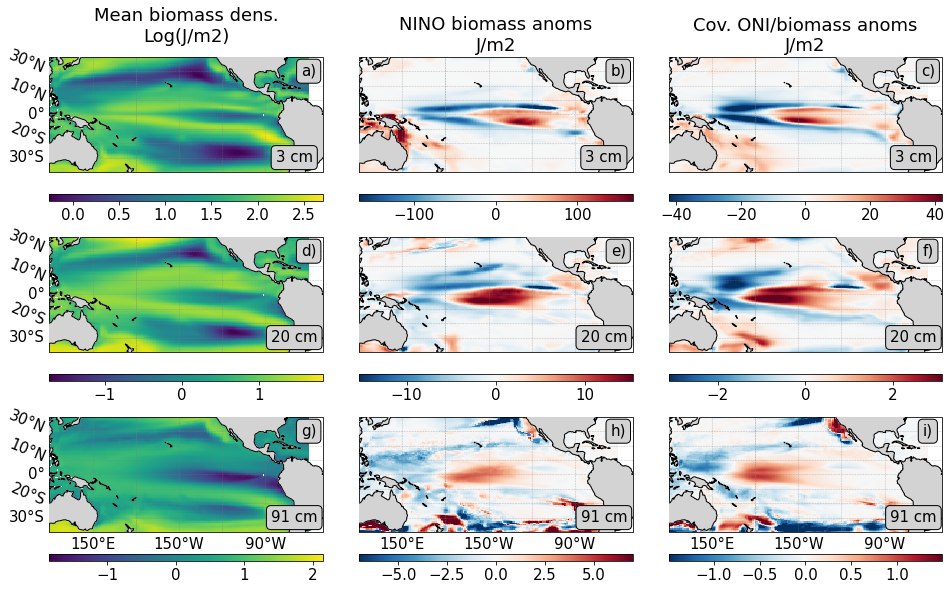
\includegraphics[scale=0.4]{figs/map_mean_anom_OND_97.png}	
	\caption{OND-NINO anomalies (left column) and covariance of fish biomass anomalies with the ONI index (right column) for small (upper line), intermediate (middle line) and large sizes (lower line). Black contours show the contours of mean fish biomass density (log-scale).}	
	\label{fig:mean_ond97_ape}
\end{figure}

%The patterns of the functional response and growth rates are very different for small sizes (figures YYY.a and YYY.d). The former shows negative anomalies on the central Pacific during the onset of El Nino conditions, presumably due to the concomitant reduction of plankton concentration (figure YYY.b). Interestingly, no anomalies are found in the eastern basin, due to compensating effects of warming temperatures and reduced plankton concentrations. The growth rate shows a pattern that is very similar to the temperature anomalies (Fig. XXX.a), indicating the dominance of temperature on the growth rate. The mortality rate (Fig. YYY.g) shows a pattern that is consistent with the increased biomass of intermediate epipelagics (XXX.b), which predate on small ones.  Besides, growth rate anomalies superimpose well on the small biomass anomalies (black contours in Fig. YYY.d), hence suggesting that the increased biomass during the El Nino conditions is triggered by enhanced growth associated with warmer temperature, despite a dampening effect of increased mortality rates.
%For intermediate sizes, the functional response and the growth rate show very similar anomalies, hence suggesting that they both are driven by the same factors. Both show positive anomalies during the onset of El Nino between 200E and 250E, presumably induced by the temperature warming that favours both the growth and search rates. Then negative anomalies occur, which are westward shifted relative to the positive ones. These negative anomalies are likely induced by the cooling associated with the La Nina conditions reinforced by the reduced small fish biomass that appears near 200E, as shown in Fig. XXX.d. Mortality rates anomalies are consistent with the increase of large fish biomass (Fig. XXX.f). Comparing the different fields, we can suggest that the increased fish biomass that appears on the central Pacific in early 1997 is first dominated by advective processes, which returns a similar pattern (fig YYY.k). Then, during the El Nino peak, the increased biomass of intermediate fish is driven by both an increased growth rate and an increased functional response, which are induced by warmer temperatures and more food available (more small epipelagic fishes, Fig. XXX.d).

%\subsection{Generalisation}
%
%In order to see if ecosystem response to the 97 El Nino event is representative, the covariance between fish biomass anomalies and the ONI index have been computed, following the methodology described in section \ref{sec:cov}. The maps are presented in Fig\ref{fig:ape_cov}.
%
%\begin{figure}
%	\centering
%	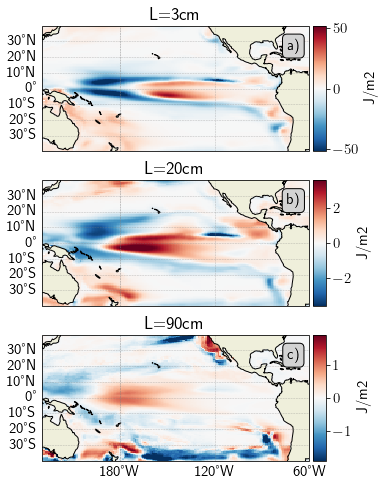
\includegraphics[scale=0.6]{figs/fig7.png}	
%	\caption{Covariance maps between the ONI index and the vertically integrated fish biomass anomalies for small (a), intermediate (b) and large (c) sizes.}	
%	\label{fig:ape_cov}
%\end{figure}
%
%The covariance patterns are very similar to the biomass anomalies depicted in Fig\ref{fig:mean_ond97_ape}, therefore suggesting that the mechanisms described in the above  apply to the general case. However, we note that the covariance patterns are westward shifted compared to the fish biomass anomalies. 
%
%This westward shift might be explained by the fact that when performing covariance anomalies, different El Nino events (Easter Pacific El Nino, Central Pacific El Nino) and La Nina events are considered, which ultimately impacts the global view of fish biomass response to ENSO variability.


%In this section, the interannual response of epipelagics to ENSO variability is investigated using covariance analysis. The left panels of Figure 3. show the yearly mean vertically integrated fish biomass over the entire simulation for the three different size classes. For small sizes (Figure 3a), the fish biomass is concentrated at around 10° S and 10 ° N in the central Pacific and close to the equator in the western Pacific. High biomass concentration is also found east of 90° W, off the coasts of Chile. As size increases, the equatorial "blue spot" extends meridionnally and to the west. This pattern is mostly driven by the active and passive advection of fishes in the Apecosm model (REF). Without advection, the biomass will be concentrated at the equator, where the plankton concentration is the maximum.
%
%Covariance maps between vertically integrated fish biomass and the winter ONI index are shown in the right panels of Figure 3. Small epipelagics show negative anomalies in the Western Equatorial Pacific and positive anomalies in the Central Equatorial Pacific. This pattern can be interpreted as an eastern displacement of the mean biomass in the Western Pacific. Similar dipolar patterns are also obtained for intermediate and large sizes, but the anomalies westward shifted as size increases. This can be interpreted, as for small sizes, by a westward shift of fish biomass during positive El Niño phases. The same results have been obtained when the covariance analysis is performed on monthly anomalies (not shown).


In order to insure that our composite of extreme El Nino events give a robust view of the response of fish biomass to ENSO, covariance maps are computed between the monthly ONI index and the detrended fish biomass anomalies over the 1958-2018 period (right column of Fig\ref{fig:mean_ond97_ape}). The El Nino composites and the covariance maps are very similar, despite anomalies slightly shifted westward and lower amplitudes for the covariance maps compared to the composites. These  differences are due to the fact that covariance analysis includes Central Pacific (i.e. Modoki) El Nino events (such as the 1986, 1991, 1994, 2002, 2004 and 2009 events) and La Nina events, whose signature is not opposite to Eastern Pacific events. Nevertheless, the very good agreement between the covariance maps and the El Nino composites suggests that our focus on the three major events gives a robust view of fish biomass response to ENSO.